\documentclass[preview]{standalone}

\usepackage{cancel}
\usepackage{tikz}

\begin{document}
\begin{figure}[b]
    \centering
    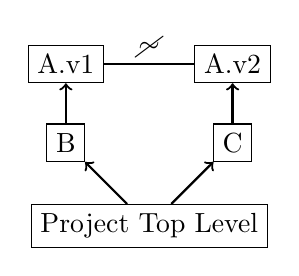
\begin{tikzpicture}
        \node [draw] (ptl) at (0,0) [align=center] {Project Top Level};
        \node [draw] [above left  of=ptl] [yshift=10] [xshift=-10]  [align=center] (B)  {B};
        \node [draw] [above right of=ptl] [yshift=10] [xshift=10]  [align=center] (C)  {C};
        \node [draw] [above       of=B]   [yshift=0]  [xshift=0]  [align=center] (A1) {A.v1};
        \node [draw] [above       of=C]   [yshift=0]  [xshift=0] [align=center] (A2) {A.v2};

        \draw[->] [black, thick] (ptl) -- (B);
        \draw[->] [black, thick] (ptl) -- (C);
        \draw[->] [black, thick] (B)   -- (A1);
        \draw[->] [black, thick] (C)   -- (A2);
        \draw     [black, thick] (A1)  -- (A2);
        \draw (A1) -- (A2) node [midway, above, sloped] (TextNode) {$\cancel{\sim}$};
    \end{tikzpicture}
\end{figure}

\end{document}